\chapter{Scenarios and Projects}
\label{ch:scenariosprojects}
% ##################################################################################################################

\hfill \textbf{Authors:} Andreas Horni, Benjamin Kickh�fer, Dominik Ziemke

\begin{center} 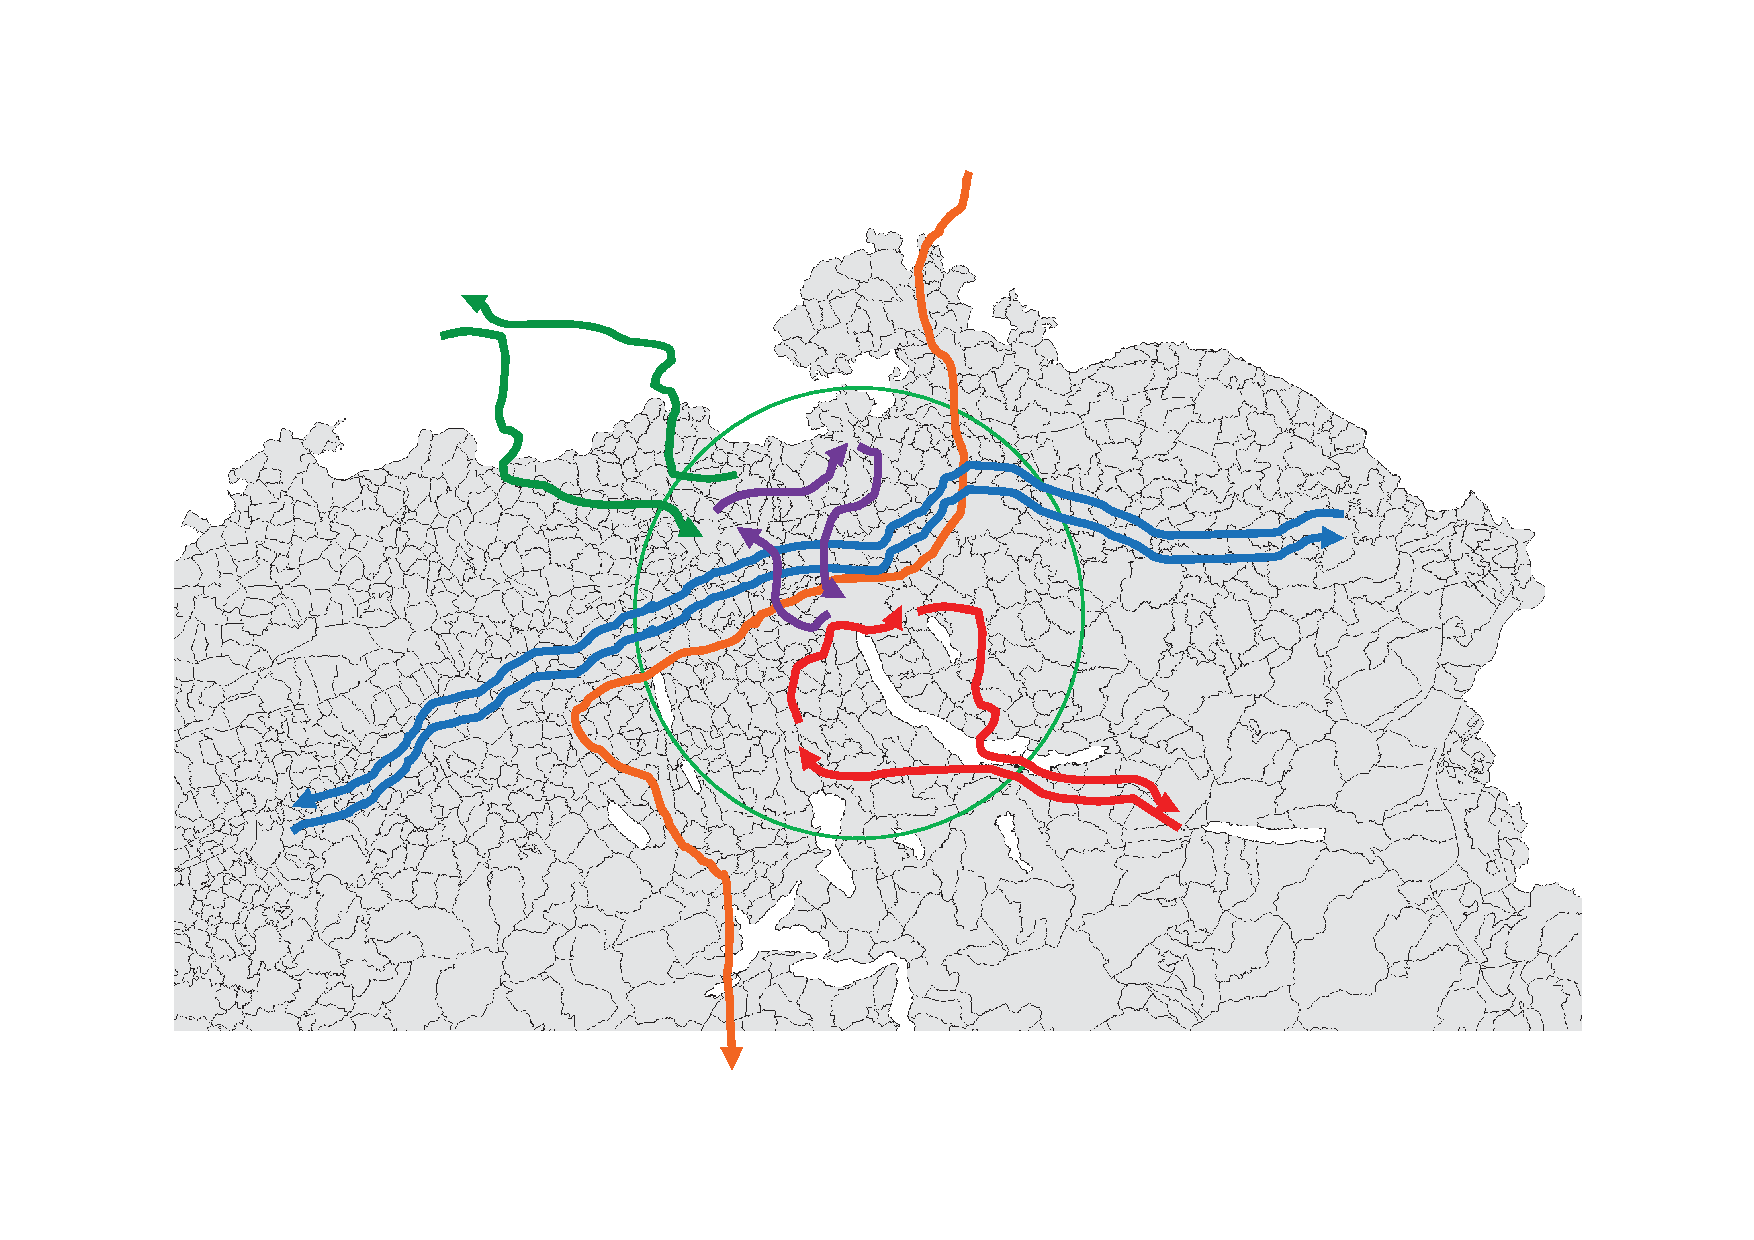
\includegraphics[width=0.7\textwidth, angle=0]{using/figures/zh} \end{center}

% ##################################################################################################################
This chapter summarizes available MATSim scenarios and projects based on MATSim (see also \citet[][]{MATSIM-T-Scenarios_Webpage_2014}). Most scenarios are not public due to privacy issues. However, knowing about the methods used for their creation and problems faced thereby might significantly support the building of new scenarios. 

Scenarios are growing continuously. Here, the latest used version is reported.

Different levels of MATSim involvement are possible. For some regions and projects, MATSim is, for example, only used for traffic assignment whereas for others the complete demand is endogenously handled. Couplings with other forecasting models for transport demand generation have been successfully applied such as the coupling with TASHA for Toronto or the combination of MATSim with the activity-based transport model of Tel Aviv.

% ##################################################################################################################
\section{Scenarios}
This section reports about the study area, demand and supply generation, ...
Utility function is described in Section \ref{sec:utfextensions}.

%- region description (characteristics, stats, ...)
%- population (popgen, Balmi plug together)
%- facilities
%- network
%- utility function (estimated, how derived)
%- pt (simulated, pseudo pt)
%- modes
%- freight (siehe keynotes Kai)
%- border crossers/boundary effects
%
%data sources
%methods applied
%
%- special problems faced \& solutions found
%
%- simulation quality
%- calibration \& validation (+available data)
%
%- purpose and sponsor/client
%- associated projects -> see Section \ref{sec:projects}
%
%- specialties: parataxis in Gauteng, connections to other sims (Toronto, Tel-Aviv)

% ==================================================================================================================
% ##################################################################################################################
\chapter{Switzerland}
\label{ch:switzerland-scenario}
\hfill \textbf{Author:} Andreas Horni

\editdone{This text has undergone the professional edit. Please no grammatical changes anymore! They are most-probably wrong.}

% ##################################################################################################################
The Switzerland scenario was initially created for the project Westumfahrung \citep[][]{BalmerEtAl_ResRep_bdktzrh_2009} and serves as the base for the very frequently used Zürich scenario (Chapter~\ref{ch:zhscenario}). 

Two main branches can be distinguished. The first, older one is based on a one-to-one translation of the Swiss population census \citep[][]{BfS_VZ_2000}; the second applies approaches from the \gls{ipf} family, reported by \citet[][]{MuellerKAxhausen_TechRep_IVT_2013, Mueller_unpub_LATSIS_2012, Mueller_unpub_ETC_2011, Mueller_unpub_STRC_2011, Mueller_unpub_IATBR_2012} to generate population.

The scenario's study area covered all of Switzerland. Due to administrative borders, no demand and supply data were available for adjoining countries, which, then and now, leads to boundary effects; studies focusing on Swiss border areas are difficult.

The population was derived from the Swiss Census of Population~2000 \citep[][]{BfS_VZ_2000}. The complete Swiss population was modeled, resulting in around 7.5\,million agents. 

This population's home locations were given at hectare level and work locations were specified at municipality level from commuter matrices, a component of the Swiss Census of Population~2000 \citep[][p.35]{BalmerEtAl_ResRep_bdktzrh_2009}. A very good overview, in German, of the population generation, its initial individual demand and activity locations can be found in \citet{MeisterEtAl_SVT_2009}. Further information is given in \citet[][]{CiariEtAl_STRC_2008, MeisterEtAl_WCTRS_2010, BalmerEtAl_ResRep_bdktzrh_2009, BalmerEtAl_ResRep_datapuls_2010, BalmerEtAl_HEUREKA_2008}.

Travel demand was basically taken from the 2000 and 2005 National Travel Surveys \citep[][]{BfS-MZ2005_manual_2006} (Swiss microcensus), although this sample substantially underestimated freight traffic and ignored cross-border traffic of non-Swiss residents. Freight traffic for Switzerland was missing at this time (except Zürich, see next chapter). Cross-border traffic was derived from mode-specific, hourly origin-destination matrices given by \citet[][]{VrticEtAl_ResRep_UVEK_2007}. These were disaggregated to around 600\,000 individual \gls{matsim} plans for the whole country, which contain the cross-border traffic originating \emph{outside} Switzerland. Non-Swiss, cross-border traffic starting in Switzerland was supposed to be negligible. 

The activity location data set, comprising home, work, education, shopping and leisure locations, was also derived from the 2000~Swiss Census of Population and the 2001~Federal Enterprise Census \citep[][]{SwissEnterpriseCensus_manual_2001}, providing hectare level information. Facility generation was described in \citet[][p.33]{BalmerEtAl_ResRep_bdktzrh_2009}.

For car traffic, navigation networks from Teleatlas \citep[][]{MultiNet_Webpage_2010} and \gls{navteq} \citep[][]{Navteq_2011} were available. The most-used network was the planning network derived from from the Swiss National Transport Model \citep[][]{VrticEtAl_BiegerEtAl_2003}.

The public transport simulation network was derived from the National Transport Model of the \gls{uvek}, described by \citet[][]{VrticFroehlich_ResRep_UVEK_2010}. 

The scenario simulated car and public transport; schedules for public transport were given at the municipality level. Fine-granular schedules were not available then, but were in preparation. The modes walk and bike were usually ``\gls{teleported}''. 

Calibration was mainly performed for modal split and distance distributions; utility function values were set accordingly.

For validation, count data on city level, cantonal level and national level \citep[][]{ASTRA_Webpage_2006} were available from various sources, resulting in 600\,links measured for Switzerland. An average working day (Monday to Thursday, excluding public holidays) was used for comparisons in current projects.

% ##################################################################################################################
 ok

% ==================================================================================================================
% ##################################################################################################################
\section{Zürich}
\label{sec:zhscenario}
\hfill \textbf{Author:} Andreas Horni

\editdone{This text has undergone the professional edit. Please no grammatical changes anymore! They are most-probably wrong.}

% ##################################################################################################################
The \gls{matsim} team frequently uses the Zürich scenario, based on the Switzerland scenario described above. The Zürich scenario, however, was more detailed; it was enhanced by data available only for the smaller region; \eg traffic light data or freight demand data was only included for Zürich city and the canton. It is under continuous development, calibration and validation and has been applied in numerous projects, serving as a real-world research example.   

\citet{HorniEtAl_TechRep_IVT_2011_a} provided a technical overview of the first scenario branch; \citet[][]{BalmerEtAl_ResRep_bdktzrh_2009} described its generation for the ``Westumfahrung'' project . 

The study area was delineated by a circle, with a 30\,kilometer radius around Bellevue, a central and prominent Zürich location. This delineation led to two versions,  the \emph{Zürich diluted scenario} and the \emph{Zürich cut scenario}. For the first, all agents crossing the study area during the simulated day were considered (Figure~\ref{fig:zurichScenario}), resulting in almost 2\,million agents. For the second, only agents remaining in this area the whole day were modeled. The \emph{Zürich cut scenario} was employed as an experiment in \citet[][]{Hackney_PhDThesis_2009}, but using the \emph{Zürich diluted scenario} for production runs is preferable.

Demand was taken directly from the Swiss model; freight traffic was also added to the Zürich scenario, as follows. Canton Zürich raw freight traffic data was taken from the \gls{kvmzh}, provided by \citet{AMV_Webpage_2011} and documented in \citet[][]{GottardiBuergler_SV_1999}. Zonal level matrices were disaggregated to single \gls{matsim} plans \citep[][]{ShahM_TechRep_IVT_2010}. Matrices for small delivery and heavy trucks were combined into one activity called \emph{freight}. An additional 180\,000 agents were generated for the Zürich region.

For the diluted Zürich scenario, all Swiss facilities, as described above, were used as activity locations. For the diluted scenario, the networks were not thinned out. For  public transport simulation, network and transport schedules were derived from the \gls{kvmzh}. Walk and bike modes were ``teleported''. 

Calibration was mainly done for modal split and distance distributions and utility function values set accordingly.

For validation, count data on city level, cantonal level and national level \citep[][]{ASTRA_Webpage_2006} were available from various sources, resulting in 123\,links measured for the Zürich inner city, delineated by a 12\,kilometer radius around Bellevue. The reduced count analysis radius was applied to reduce boundary effects resulting from demand reduction outside the 30\,kilometer radius study area. An average working day (Monday to Thursday, excluding public holidays) was used for comparison in current scenarios.

Some traffic signal data was available for Zürich city \citep[][]{STAPOZH-DAV_unpub_gtZH_2008}; this was integrated for the Westumfahrung project.
%
\createfigure%
{The diluted Zürich scenario}%
{The diluted Zürich scenario}%
{\label{fig:zurichScenario}}%
{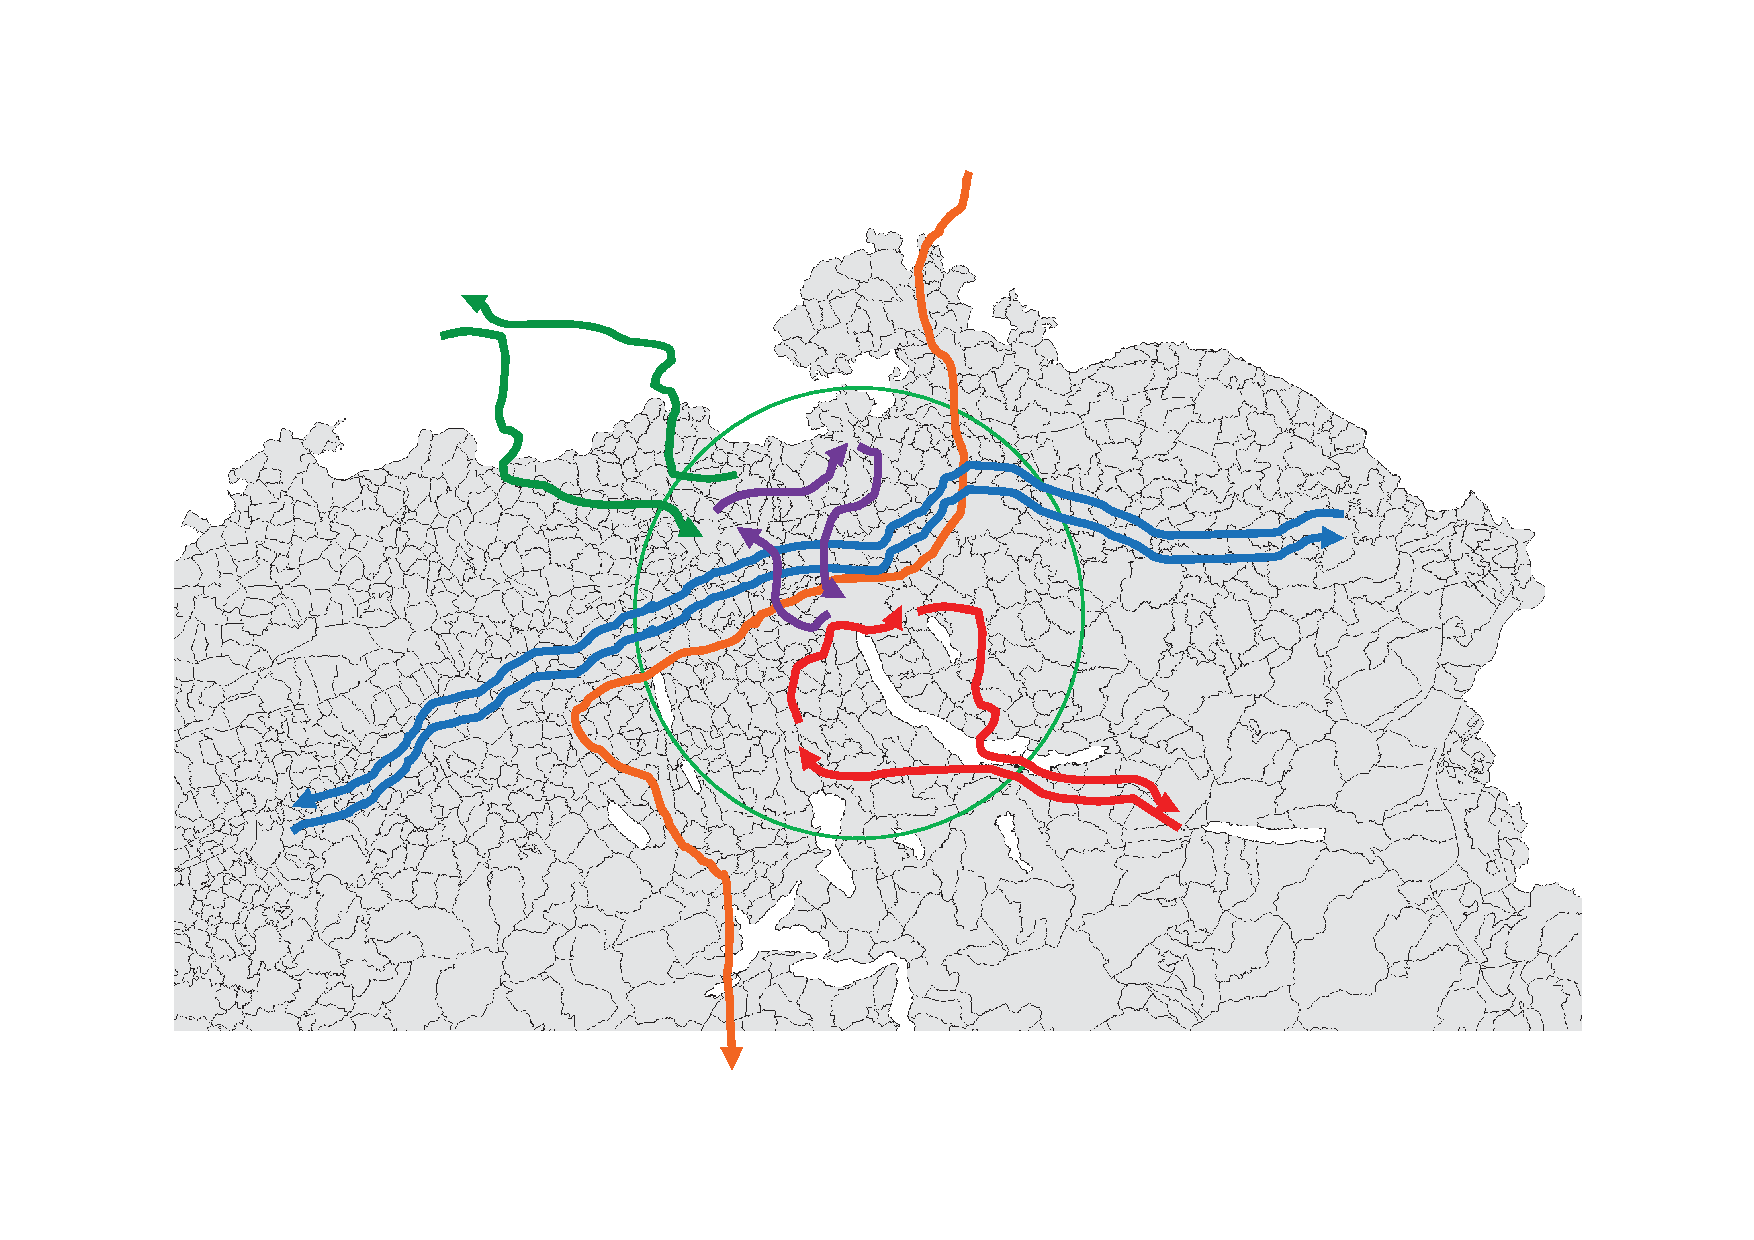
\includegraphics[width=0.99\textwidth, angle=0]{using/figures/zh.pdf}}%
{}

% ##################################################################################################################
 ok

% ==================================================================================================================
% !TeX root = ../../main.tex
% ##################################################################################################################
\section{Berlin I: BVG Scenario}
\label{ch:scenarios:berlinI}
\hfill \textbf{Author:} Andreas Neumann

\citep[][p.67ff]{Balmer_PhDThesis_2007}

coupling with Visum BVG \\
Marcel: IATBR \\


The Berliner Verkehrsbetriebe (BVG) is Berlin's main public transport company
and runs all kind of services with the exception of the S-Bahn urban rail
system. This includes bus services, the subway network, the largest tram network
of Germany as well as ferry services. The bus network consists of 149
different lines, 6468 directed stops and a vehicle fleet of 1316 buses \citep{BVG2012}.
In total, about 937~million trips were served by BVG in 2012,
41\,\% of them by bus.

% start excerpt from the paper
With the opening of the new international airport of Berlin and Brandenburg BER,
Berlin is expecting some major changes in travel demand. Especially, the
existing airport Tegel, currently exclusively served by buses operated by BVG,
will cease operations. BVG had thus a large interest in a new transport model
for the Berlin area. Due to the big changes, the model should not only deliver
the basis for future planning of the regional transport system, but has to
provide detailed information about passenger flows of different user groups as
well. Such user group specific analyses are considered of high importance for
the BVG in order to provide a basis for their future business strategies, which
is why an agent-based model was specifically requested. Two scenarios were
actually asked for, one for the year 2008 (actual state), and one for the year
2015 (prediction). To fulfill the needs mentioned above, the team of 
\citet{PTV2013}, \citet{Senozon2013} and \citet{VSP2013} at Technische Universit{\"a}t Berlin (TU Berlin)
offered a combined model consisting of both a static macroscopic model built with
PTV VISUM \citep{VISUM2013} as well as an integrated activity-based demand and
dynamic traffic assignment model built with MATSim. During
the project, attention was given that both models were based on the same data
sources and that both modeling processes interact with each other to allow data
exchange between the two models.
% end excerpt from the paper

In
brief, the model contains about 115,000 links, % 113269
about 15,000 directed stops, % 14902
6.0~million agents, % 4422012 (sex) 5992771 (/person)
and 539 public transport lines operated by BVG and other companies of the city
of Berlin and the state of Brandenburg. Among others the model features the transport modes Besides the transport modes car, For a more in-depth description of the
model, its generation and its calibration, the reader is referred to the work of
\cite{NeumannEtAl2014IatbrPtBerlinBook}. The model has been extensively been used in \citet[][Ch 7/8]{Neumann2014PhD} for the development of the minibus module of Section~\ref{sec:paratransit}.



% ################################################################################################################## ok

% ==================================================================================================================
% ##################################################################################################################
\section{Berlin II: CEMDAP-MATSim-Cadyts Scenario}
\label{sec:berlinII}
\hfill \textbf{Author:} Dominik Ziemke

% ##################################################################################################################

As explained in section ?????, transport modeling can be considered as the representation of the interaction of transport demand (i.e. people and goods being transported) and transport supply (i.e. transport infrastructure and services) in the transport system. Depending on the application of innovative strategy modules (see section ?????), MATSim accounts for the adaption of transport demand to transport supply \citep{Balmer2007phd}. It is, therefore, crucial to distinguish choice dimensions, which may be adapted during the modeling process (via the application of innovative strategy modules, see section....) and choice dimension whose initial properties are assumed to be correct (e.g. mode shares have to be initially correct in a scenario where the choice of transport modes is not modeled). In the latter case, it is important that respective properties of the transport demand are correct at the start of the simulation (see section Data Requirements - Demand???).

In order to model these properties of the initial demand correctly, suitable data are needed. A widely utilized source of such data are travel diaries, which contain sequences of departure times, mode choice decisions, and activity locations.
%A disadvantage of using trip diaries is, however, that all information that is taken from the diaries is by definition not sensitive to policy measures. Also, trip diaries are normally only available for a very small fraction of the population. Another drawback is that, in Germany and the U.S. (and many other parts of the world), the geo-coding of the activity location is considered sensitive information under privacy legislation, and thus increasingly difficult to obtain (cite ZiemkeNagelBhat2015).
Many contents of this data source, in particular information concerning locations, are, however, in many parts of the world (e.g. in Germany and the United States) considered sensitive in terms of data privacy legislation and thus increasingly difficult to obtain and to process \citep{ ZiemkeNagelBhat2015IntegratingCemdapMatsimTransferabilityTRB}.

The \textit{Berlin II scenario} (also referred to as the \textit{CEMDAP-MATSim-Cadyts scenario} according to applied models in its setup) is the outcome of an alternative approach that relies exclusively on input data that are freely available and easy to obtain. The starting point for the Berlin II scenario are publicly available commuting matrices which contain home and work places of socially-secured workers on the municipality level. Based on this information, it is possible to model morning and evening commuting peaks.

In order to obtain a demand representation of the full population, two further major modeling steps are required. First, in cases (like in the Berlin case, see below), where the spatial resolution of the commuter matrix is quite coarse, a method to attain origin-destination information at a higher resolution is needed. Second, there needs to be a procedure to model secondary activities, i.e. all other activities that go beyond home and work activities.

The necessity of the first step becomes obvious when looking at the German case, where, for instance, all of the city of Berlin, with 3.4 million inhabitants, is represented by exactly one zone \citep{BA2010Pendlerstatistik}. In the U.S., commuting matrices are typically available only at a county-to-county level. Since such location-aggregation-based matrices may become the rule rather than the exception in privacy-sensitive societies, a (generalizable) method to attain origin-destination information at a higher resolution is needed \citep{ ZiemkeNagelBhat2015IntegratingCemdapMatsimTransferabilityTRB}. The standard solution would be to estimate an activity location choice model. This, however, is difficult if no trip data to estimate the model is available. OD matrix estimation studies \citep{ZuylenWillumsenMatrix-from-cnts} suggest that traffic counts may be used to make an initially rough OD matrix more appropriate for a region. As MATSim is not based on OD flows (see section ????), but on full daily plans, the issue becomes whether there is a procedure to update these initial full daily plans using traffic counts. In the approach to create the Berlin II scenario, a procedure proposed by Flötteröd et al. \citep{FloetteroedBierlaireNagel2010Bayesian} and implemented in the software Cadyts (Calibration of Dynamic Traffic Simulations \citep{Floetteroed2010Manual110}) is applied for this task. Specifically, random draws of possible home and work locations within the home or work municipality given by the commuter matrix are taken. Various MATSim plans each containing one pair of home and work locations are created for each agent. Then, the Cadyts calibration procedure is applied within the iterative MATSim simulation to select those plans, and thus also those locations, which appear more plausible with regard to given traffic counts.

As stated above, however, full daily plans (as opposed to mere home-work-home comuting patterns) are needed. Therefore, the second aforementioned additional modeling step, the modeling of secondary activities for each individual in the region, needs to be addressed. For the Berlin II scenario, the Comprehensive Econometric Microsimulator for Daily Activity-Travel Patterns \citep{BhatEtAl2008CEMDAPUserManual} is used to generate initial complete daily plans for each individual. One the one hand, however, no CEMDAP parameter set is available for Berlin. On the other hand and more importantly, one major goal of the study creating the Berlin II scenario was to show is generalizability \citep{ ZiemkeNagelBhat2015IntegratingCemdapMatsimTransferabilityTRB}. So, the model parameters of CEMDAP estimated for the Los Angeles region (the estimation context) are retained, and then used to generate the initial plans for individuals in Berlin (the application context in the current paper) based on Berlin demographic data.

To sum up, home and work municipalities are taken from the commuter matrix. Within these municipalities, a set of (more precisely spatially defined) potential home and work locations are randomly chosen for each agent. Full daily plans incorporating the various potential locations of each agent are generated with CEMDAP based on a parameter set from another region and local demographic data.

Then, the Cadyts calibration procedure is used to select those initial full daily plans that are most consistent with Berlin traffic count data. In other studies, Cadyts has already been applied to update route choice predictions, both for car \citep{FloetteroedChenEtAl2011BehavioralCalibAndAna} and for public transit \citep{MoyoNagel2013ptNetCalibrationABMTPO}. However, it has not been used to update full daily activity-travel plans, as it has been done in the procedure that created the Berlin II scenario. 

As a result, the Berlin II scenario, is an activity-plan-based MATSim transport model for Berlin that is exclusively based on freely or easily available data. If a commuter matrix, some basic demographics of the population, and traffic counts (or theoretically another suitable data source to run the calibration procedure on) are available for a particular regional context, the approach used to create the Berlin II scenario can be transfered to this context. In fact, the Berlin II scenario itself has to be seen as a \textit{transferred model} because the initial plans generated by CEMDAP are based on parameter estimates from another geographic region (namely the Los Angeles area).

Through a validation based on the Berlin 2008 SrV \textit{System repräsentativer Verkehrserhebungen}, an extensive, regularly conducted travel survey, the quality of the created transport demand representation has been successfully tested. So far, the Berlin II scenario exists for a 1\%{} and a 10\%{} population sample of all persons, i.e. also non socially-secured workers and also non-working people, aged 18 and above for the study region. Currently, only motorized traffic is considered. Stability tests, showing that agents' daily plans keep being chosen when the Cadyts calibration functionality is switched of, have been successfully carried out. This can be seen as a clear indication that the scenario is applicable for policy studies in a meaningful way.

Further improvements like the addition of public transport and a more realistic representation of the population are planned. Moreover, similar approaches of integrating activity-travel pattern generators (e.g. the FEATHERS model, cite?????) with MATSim as a transport simulation are planned.

\ah{NOTES: to be removed:
AN: Szenario entstand aus einer Arbeit zur Nachfragegenerierung. Würde also auch in einen conceptual part passen, anderer Ansatz als die meisten anderen Szenarien ("datensparsam"), Integration von CEMDAP (Modell zur Aktivitätenkettenerzeugung)

Auch link auf Cadyts.

Aktivitätenkettenerzeugung: ähnlich zu Tel Aviv Modell

FEATHERS am Beginn -> Vortrag Wiepersdorf
}

% ################################################################################################################## ok

% ==================================================================================================================
% ##################################################################################################################
\section{Singapore}
\label{sec:singapore}
\hfill \textbf{Author:} Alexander Erath, Artem Chakirov

% ##################################################################################################################
The MATSim Singapore scenario \citet[][]{ErathEtAl_TechRep_FCL_forth} was implemented and is maintained at the Future Cities Laboratory, a research program of the Singapore-ETH Centre for Global Environmental Sustainability (SEC) and part of Singapore's National Research Foundation CREATE (Campus for Excellence and Technological Enterprise). The scenario covers the whole area of Singapore with a population of approximately 5 million inhabitants and includes traffic from and to neighboring Malaysia. Singapore provides an excellent study case for an agent- and activity based modeling approach: a fairly densely populated city with an extensive public transport infrastructure and advanced transportation and pricing policies. 

% ====================================================================================================
\subsection{Demand}
In the absence of a full-population census for Singapore, a synthetic population is generated based on data from the Household Interview Travel Survey (HITS) 2008 \citep[][]{Choi_JOUR_2010} and population breakdowns of Singapore’s population census 2010. The synthetic population was derived using the fitting and sampling method \citep{MuellerKAxhausen_TRB_2011}, where a reference sample of household and person records  is weighted using an iterative proportional fitting (IPF) technique, until the weighted sample matches marginal control totals from the census. In our case, the reference sample is the records form the travel survey, and the fitting technique is the entropy optimization method proposed by \citet[][]{BarGeraEtAl_TRB_2009}, implemented by Kirill Müller, IVT, ETH Zürich. Then the reference sample records are replicated through weighted sampling until the population total is met. 
 
Car ownership is modeled on a household level and driving licenses are assigned to individuals, using discrete choice methods. Given the high taxation of cars in Singapore, the model reflects that car ownership is much lower than in other developed nations. The model presented in \citet[][]{VanEggermondEtAl_IATBR_2012} includes not only socio-economic but also spatial variables and has proven to be essential to the MATSim Singapore model, leading to accurate mode choice and mode share predictions. 

Activity locations are defined on the level of individual buildings, with the information on building and facility types compiled from various sources such as the land-use master plan \citep[][]{URA_Rep_URA_2008}, government websites and online directories as well as points of interest information provided by NAVTEQ. In the absence of a business census, an innovative approach for identification of locations and corresponding number of work places has been developed. It draws from the full smart card data record of public transport journeys and enriches it with information on land-use and estimates of building floor space. In a first step, a probabilistic model is applied to a daily record of public transport journeys in order to identify types of activities performed between two subsequent public transport trips. Estimated and calibrated using HITS 2008 records, the model combines variables such as time of day, activity duration and land-use around each stop or station to ensure an accurate differentiation between home, work or other activities. After accounting for mode shares in 53\,different zones, an optimization technique employing accessibility computation is applied in order to distribute work activities to individual buildings. More details on the newly developed methodology and its practical application are reported in \citet[][]{ChakirovErath_IATBR_2012} and \citet[][]{OrdonezErath_TRR_2013}. 

The assignment of households to buildings is performed using detailed information on residential developments: for public housing which represent about 80\,\% of Singapore's residential building stock, information on the distribution of different dwell types is employed, while for privately owned condominiums, only information on the number of apartments per building is available. Work locations are assigned using a zone-based gravity model that uses the prior estimated number of work activities in each building as additional information for the distribution of workplaces within each zone. Activity chains are assigned based on their observed frequency in HITS, taking into account key socio-demographic parameters such as sex, age, occupation and income. Activity chains of type home~--~work~--~home are by far the most frequent, accounting for approximately 50\,\% of the trips.
Freight and cross border traffic as well as tourist travel demand are derived based on a set of origin destination matrices provided by the Singapore Land Transport Authority (LTA). These matrices are converted into special daily plans. Information on the temporal distribution of trips for freight is derived from loop detector data for freight and temporal attraction profiles of major tourist sites.

% ====================================================================================================
\subsection{Supply}
Using a semi-automatic map-matching algorithm~\ref{sec:networkeditor-singapore} a high-resolution navigation network provided by NAVTEQ is map-matched to and enhanced with lane and capacity information from the Land Transport Authority's (LTA) planning network. In absence of access to traffic signal cycle time data, traffic lights are not specifically modeled. Extensive attention was paid to the modeling of public transport due to the the importance of interaction between private and public transport in Singapore’s context of high density and limited space. Simulating dynamic effects such as bus bunching is crucial for obtaining realistic travel times and mode shares. Public transport network and schedule data provided by LTA includes bus and train routes,  as well as the location of stops and stations. This information has been matched to the road network using yet another map-matching algorithm presented by \citet[][]{Ordonez_HKSTS_2011, Ordonez_Webpage_2011_4}. More recently, the scenario got updated by using public transport schedule data as derived from public transport smart card data records \citet[][]{Fourie_TechRep_FCL_2014}. Such schedule information accounts for the actual vehicle dispatch frequencies and headways, which undergo continuous adjustments and in some cases can substantially deviate from the published schedule. Furthermore, additional features of the public transport simulation in Singapore’s model include advanced bus dwell time model \citep[][]{SunEtAl_TransResA_2014} as well as an approximation of the distance based public transport fare scheme.

Other modes, specifically walking and cycling are "teleported" with constant travel speeds and without any interaction with other users. 

% ====================================================================================================
\subsection{Behavioral parameters}
The behavioral parameters, specific to Singapore's context have been borrowed form the study by \citet[][]{LTA_unpub_2009} and used in conjunction with the widely applied Charypar-Nagel function for activity scoring \citet[][]{CharyparNagel2005ga4acts}. Thereby same parameters have been used for all agents, neglecting heterogeneity of user preferences and values of time in the initial scenario implementation. Furthermore, no additional crowding penalties accounting for travelers' discomfort have been considered at this stage and the effects of public transport overcrowding are only taken into account with the physical vehicle capacity limitations as well as its implications on dwell time and occurrence of the bus bunching phenomenon. 

% ====================================================================================================
\subsection{Policy}
The MATSim model for Singapore also includes the Electronic Road Pricing (ERP) scheme featuring time and vehicle dependent road pricing. Based on two data sets indicating the location and time dependent price levels, prevailing tolls are specified for 73\,network links where toll gantries are installed as of February, 2012. To account for the widely available dedicated bus lanes, additional links that are attributed to be used exclusively by buses have been added to the network. The capacity of the respective existing links has been reduced accordingly, even if in some cases the exclusive use of dedicated lanes by buses is granted during the peak hours only. Such a simplified setup, insensitive to the time dynamic operation of the dedicated lanes, leads to an underestimation of actual road capacity during periods when bus lanes are also open to other motorized traffic. However, as most links featuring bus lanes consist of three or more lanes, the effect on modeled traffic conditions during off-peak hours appears to be low.

% ====================================================================================================
\subsection{Calibration and validation}
Road usage data is available for around 200\, 
%\textbf{EXACT 200?} 
count stations in hourly intervals. The availability of public transport smart card data provides an additional dimension for validation. In particular opening of new mass rapid transit (MRT) lines since setting up the model in 2012 presents a unique opportunity for comparison the observed ridership with predicted ridership in the model. However, systematic calibration and detailed validation are yet to be conducted.

% ##################################################################################################################

% ==================================================================================================================
% ##################################################################################################################
\subsection{Munich, Germany}
\label{ch:scenarios:munich}
\hfill \textbf{Author:} Benjamin Kickh\"ofer

The \acrshort{matsim} scenario for the Munich metropolitan area was set up during the year 2010.%
%
\footnote{
%
The most detailed descriptions of the scenario can be found in \citet{KickhoeferEtAl_VanoutriveVerhetsel_2013} and \citet{Kickhoefer_PhDThesis_2014}.
%
}
%
The main goal was, and still is, the simulation of local air pollutant and global greenhouse gas emissions, and how their levels change with respect to different policy measures -- on aggregated and spatially disaggregated level. The scenario was therefore used for the development and testing of the \gls{emt} (see Ch.~\ref{ch:emissions}).

Network information from \acrshort{visum} was converted into \acrshort{matsim} format, resulting in a network of 17'888 nodes and 41'942 links.
%
This transport supply was then linked to travel demand from different sources: an activity-based demand for inner-urban traffic from survey data was created based on "Mobility in Germany" \citep[MiD 2002,][]{FollmerEtAl_TechRep_infasDIW_2004}. This part of the synthetic population consists of roughly 1.4m individuals with detailed vehicle information for every household.
%
Commuter and reverse commuter were modeled based on data provided by the German Federal Employment Office \citep{BoehmeEigenhueller_TechRep_IAB_2006}. This part of the population consists of roughly 0.5m individuals from which 0.3m commute to Munich for work. The remaining individuals live in Munich and commute to their workplace in the surroundings of Munich.
%
Freight traffic was also introduced into the model by using data from the German Ministry for Transport \citep{ITBBVU_TechRep_2007}. This part of the population consists of roughly 0.15m freight vehicles who perform one single commercial trip per day.

The scenario has so far been used for several case studies:
%
\citet{HuelsmannEtAl_LAS_2011} used a single street corridor of the scenario to validate simulated travel times and emission levels against actual data obtained from a test vehicle.
%
\citet{KickhoeferEtAl_VanoutriveVerhetsel_2013} investigate the relationship between the price elasticities of car travel demand and those of air pollutant emissions.
%
\citet{HuelsmannEtAl_GerikeEtAl_2013} identify areas with high air pollution concentration in the city. They define these areas as 'hotspots' since the \gls{eu} limits for \gls{no2} are exceeded. The authors then incrementally raise the toll levels for passing the hotspots until they disappear in order to estimate the true avoidance costs of the \gls{eu} threshold values.
%
\citet{KickhoeferEtAl_NSE_2013} derive time-dependent vehicle-specific first-best air pollution tolls in order to create a benchmark for the evaluation of real-world policies.
%
\citet{KickhoeferKern_MobilTUM_2014} go a step beyond and calculate time-dependent vehicle-specific air pollution exposure tolls in order to correct the toll levels by \citet{KickhoeferEtAl_NSE_2013} for the number of affected individuals.



% ################################################################################################################## ok

% ==================================================================================================================
% ##################################################################################################################
\section{City of Sioux Falls, South Dakota}
\label{ch:scenarios:siouxfalls}
\hfill \textbf{Author:} Artem Chakirov

The Sioux Falls scenario represents a small scale scenario featuring realistic demand with socio-economic and demographic attributes and an integrated public transport system. Based on the  Sioux Falls road network commonly featured as a test-case in the transportation literature \citep[][]{BarGera_TNTP_Webpage_2013}, the scenario aims to provide a fully dynamic demand with heterogeneous users and a high degree of spatial resolution. It can serve as a convenient test-case for the study of different transportation policies as well as a test bed for the software extension and development. However, it is important to stress that despite the use of real world data for its generation, the scenario does not aim to replicate the real City of Sioux Falls in South Dakota, US and remains a fictitious test-case scenario. Detailed report on scenario generation and its characteristics is provided \citet[][]{ChakirovFourie_TechRep_FCL_2014} and can be found at www.matsim.org/scenario/sioux-falls. 

Often used test scenario . Not aimed at replicating the real City of Sioux Falls, South Dakota.

% --------
\paragraph{Demand:}

A realistic, socio-economically and demographically diverse demand population with  heterogeneous preferences is crucial for unlocking the full potential of an agent-based simulation. However, the generation of a disaggregated, agent-based demand description, which closely resembles reality, not only in terms of trip origins and destination, but also with respect to associating travel patterns with socio-demographic characteristics, is challenging.

In order to address this challenge in case of Sioux Falls scenario and represent the household structure, demographic profile and income distribution as realistically as possible, a synthetic population of households using entropy maximization technique is generated. It matches the aggregate distribution of demographic attributes (age, sex and household income) recorded during the 2010 US Census for the 27 census tracts inside and adjoining the city centre of Sioux Falls and is composed of household and person records taken from the (anonymous) 5-year sample (2007-2011) of the American Community Survey, covering 5.0\% of all households.

On the demand side of the activity-based model only two simple activity chains are initially included, in order to keep the scenario accessible and to facilitate interpretation and understanding of the possible effects of policies under study. Modelling only home – work – home and home – other – home activity chains, destinations are assigned using a parameter-free radiation model (Simini et al. 2012).

Activity locations are identified using the data set of real building stock provided by the City of Sioux Falls GIS division. The home location of each household is assigned randomly to a residential unit within the tract it belongs to. As no information on the real number and distribution of work places within the relevant area is easily accessible, the static OD-Matrix from LeBlanc et al. (1975) are taken as an indicator of workplace attraction for each zone. Subsequently, the assignment of work places to individual workers was performed using a parameter free radiation model presented by Simini et al. (2012).

In order to exploit the full potential of a disaggregated demand and to add another degree of realism to the scenario, a car ownership model is applied to the synthetic population of households. An ordered probit model estimated by Giuliano and Dargay (2006)based on the US Nationwide Personal Transportation Survey (NPTS) 1995. Next to socio-demographic characteristics of a household (number of adults, children, pensioners, household income), the model uses attributes of residential location (population density, public transport access and dwelling type), which allows to better account for characteristics of the Sioux-Falls scenario with its added area-wide bus network. 

% --------
\paragraph{Supply:} 

A transportation test network should ensure sufficient complexity of travellers’ choice dimensions while limiting computational effort. To this end, the Sioux Falls test network was introduced by Morlok et al. (1973) and later adapted as a benchmark and test scenario in many publications, as e.g. LeBlanc et al. (1975), Abdulaal and LeBlanc (1979a), Suwansirikul et al.  (1987), Friesz et al. (1992), Meng et al. (2001), Bar-Gera et al. (2013) to name but a few. The structure of this network captures the major arterial roads of the City of Sioux Falls, but was never intended to replicate the real city or all characteristics of its transportation system, such as travel times or mode share. The network os comprised of 76 arcs, 24 nodes and 552 origin-destination pairs. For this scenario the capacities of the roads were adjusted according to values provided by the Highway Capacity Manual (TRB, 2000) or other related research publications (e.g. Ng and Small, 2011). The public transportation network includes 5  bus lines, as initially proposed by Abdullal and LeBlanc (1979), with bus stops placed in constant distance of 600m away from each other. 

Due to the design of MATSim’s queue simulation, agents are only handled at the beginning and end of each network link, and cannot enter or leave a link along its length. Therefore, origins and destinations located along very long links will lead to a loss of spatial detail, as all origins and destinations along the length of the link are effectively assigned the same coordinate. Consequently, to improve the level of spatial detail, all links of the Sioux Falls network are evenly split into smaller links with maximal length of 500 meters each. Following this operation, the network detail increased from 27 to 282 nodes and the number of links increased from 76 to 334.

In addition to car and bus modes, walking as 'teleported' mode with constant travel speeds and without any interaction with other users is used as the non-motorized mode of transportation. 

% --------
\paragraph{Behavioural parameters:}

The behavioural parameters used in utility functions of activities and trips are based on the estimated demand model for Sydney by Tirachini, Hensher, and Rose (2012). The time-related parameters derived in their model have to be adjusted for application in the activity-based context. In order to provide a value for marginal utility of performing an activity, the travel mode with smallest disutility is set as a baseline, under the assumption that travelling with this mode is as good or as bad as idling and doing nothing. Therefore, the corresponding parameters are split into opportunity costs of time and a mode-specific disutility of travelling, as was done previously by Kickhöfer et al. (2011), Kickhöfer et al. (2013), Kaddoura et al. (2013), Kickhöfer and Nagel (2013), who employed the same parameters within their MATSim based studies. 

% --------
\paragraph{Results, drawbacks and outlook:}

The stability and performance of the Sioux Falls scenario has been tested using two set of activity timing constrains as well as 5 different random seeds. which all delivered stable and realistic results. Furthermore \citet[][]{ChakirovFourie_TechRep_FCL_2014} also investigate the existence and shape of the Macroscopic Fundamental Diagram, as demonstrated by Geroliminis and Daganzo (2007, 2008). 

However, the more recent experience has shown certain drawbacks of the coarse network representing only major arterial roads and neglecting finer neighbourhood access road network. Combined with the realistic synthetic population and high demand peaks during rush hours, the network appears to be sensible to network breakdowns under high loading conditions. 

Along with the coarse road network, the coarse level of public transport network and therewith its low level of accessibility and attraction represents another drawback, in particular relevant for simulation and evaluation of policies sensible to or requiring certain share of public transport users. 

Substituting, the original Sioux-Falls networks with its only 76 links with a finer Open Street Map network and adding additional public transport line to it, allows to address this problem, but brings another drawbacks at the same time. First, it increases time and resources for routing and dynamic queue simulation due to the significantly larger number of links and nodes present in the network. Second, the increase in total network capacity leads to the disappearance of congestion during peak hours.

The extended simulation times can be improved by using the new pseudo-simulation methodology, currently developed by Fourie (2014). The larger network capacity can be addressed by the inclusion of freight and through traffic into the scenario. 

Drawbacks: course resolution of the network
public transport is not attractive and accessible enough, especially for experiment design in european context
no freight of through traffic


% ##################################################################################################################

% ==================================================================================================================
\subsection{Gauteng \who{Joubert}}
\citep[][]{JoubertJEtAl_TRR_2010}
https://matsim.atlassian.net/wiki/display/MATPUB/South+Africa

% ==================================================================================================================
\subsection{Cape Town \who{Joubert}}
https://matsim.atlassian.net/wiki/display/MATPUB/South+Africa

% ==================================================================================================================
\subsection{Padang \who{L�mmel}}
\citep[][]{Laemmel_PhDThesis_2011}

% ==================================================================================================================
% ##################################################################################################################
\subsection{Shanghai}
\label{ch:scenarios:shanghai}
\hfill \textbf{Author:} Lun angeschrieben

\citep[][]{WangtEtAl_TRB_2013}

% --------
\paragraph{Associated projects:}

% --------
\paragraph{Study area:}

% --------
\paragraph{Population and demand generation:}

% --------
\paragraph{Activity Locations:}

% --------
\paragraph{Network:}

% --------
\paragraph{Modes:}

% --------
\paragraph{Calibration and validation:}

\ah{Simulation quality, achieved results}

% ##################################################################################################################

% ==================================================================================================================
\subsection{Toronto \who{Balmer}}
\citep[][]{GaoWEtAl_TRR_2010}

coupling with TASHA

professor Habib angefragt

% ==================================================================================================================
\subsection{Tel Aviv \who{Dobler}}
\label{sec:telavivScenario}
\citep[][]{BekhorEtAl_TRB_2011}


% ==================================================================================================================
% ##################################################################################################################
\chapter{Cottbus: Traffic Light Simulation}
\label{ch:cottbus}
\hfill \textbf{Authors:} Joschka Bischoff, Dominik Grether

\editdone{This text has undergone the professional edit. Please no grammatical changes anymore! They are most-probably wrong.}

% ##################################################################################################################
The Cottbus (Germany) scenario (Figure~\ref{fig:scenarios:cottbus_location}) is used for traffic light simulation (see Chapter~\ref{ch:signalslanes}). 
It is explained well in \citet[][pp.~87]{Grether_PhDThesis_2014}; this chapter briefly reviews the main points. 
The scenario data is generally available to the public.

The network is derived from \gls{osm} data in summer, 2010 \citep{Bischoff2010BaSylvia} and 
covers all streets within the city boundaries, as well as main roads in the surrounding Spree-Neiße administrative district . 
It is designed as a 100\,\% sample. 
The population is based on the German federal employment agency commuter statistics for both Cottbus and Spree-Neiße \citep{WiethoelterBogaiCarstensen2010IABPendlerberichtBB}. 
As such, the population has only home-work-home plans spread over the usual commuting times, resulting in two peaks, including 
33\,479 agents traveling exclusively by car. 
The scenario is generally not very busy; the area does not usually have major congestion issues.

Figure~\ref{fig:network_municipalities_cottbus_landuse} shows the network over the 
``Corine Land Cover'' landuse \citep{CorineLandCover2006Data}, provided by European Environmental Agency. 
Woods and agricultural areas are depicted; most of the region is agricultural use area.  
Virtual persons in \gls{matsim} need a geographic coordinate for their activities. 
If this coordinate is drawn randomly (solely based on municipality borders), home and work activity locations are uniformly distributed over  the area, \ie most of them in woods and fields. 
Thus, activity locations are drawn randomly in combination with land use data. 
The coordinate must be in the municipality area and for home activity, it must be located in urban fabric areas; for work locations, industrial or commercial areas are also allowed. 
The resulting home activity locations are shown in Figure~\ref{fig:cottbus_population_home}. 

The scenario contains data for 22\,traffic signals within the city center, based on the city's 2009~signal plans; junction layout is also modeled in detail. Fixed-time control data is taken from \citet{KoehlerStrehler2010SignalDemandOptimization}.  
Due to higher transport network resolution, several originally recorded fixed-time control schedules are invalid and were removed; data for 22\,junctions is available. 
Figure~\ref{fig:cottbus_network_signal_locations} shows their transport network location.  

Public transit, not part of the original scenario, is available based on 2011~schedules, although it is not currently used. 
\createfigure%
{Cottbus scenario: Geospatial location within Germany, Europe}%
{Cottbus scenario: Geospatial location within Germany, Europe}%
{\label{fig:scenarios:cottbus_location}}%
{%
  \createsubfigure%
	{Geospatial area of Brandenburg within Germany, Europe (Red); City of Berlin (Yellow)}
	{\includegraphics[width=0.49\textwidth]{./scenarios/figures/brandenburg_europe.png}}
	{\label{fig:scenarios:cottbus_brandenburg_europe}}
  \createsubfigure%
	{Geospatial area of Cottbus (Dark Red), within administrative district Spree-Neiße, Brandenburg (Light Red)}
	{\includegraphics[width=0.49\textwidth]{./scenarios/figures/brandenburg_spree_neise_cottbus.pdf}}
	{\label{fig:scenarios:cottbus_bb}}
}%
{\citet{Grether2014PhD}}

\createfigure%
{Cottbus scenario: Network and population}%
{Cottbus scenario: Network and population}%
{\label{fig:cottbus_network_population}}%
{%
  \createsubfigure%
	{Cottbus network and municipality borders}
	{\includegraphics[width=0.49\linewidth]{./scenarios/figures/2013_network_gemeinden_landuse_edit.pdf}}
	{\label{fig:network_municipalities_cottbus_landuse}}
  \createsubfigure%
	{Synthetic population for the Cottbus scenario, geospatial location of home activities}
	{\includegraphics[width=0.49\linewidth]{./scenarios/figures/2013_network_gemeinden_landuse_population_home.jpg}}
	{\label{fig:cottbus_population_home}}
}%
{Source:~\citet{Grether2014PhD}} 

\createfigure%
{Cottbus scenario: Network, area with traffic signals within the city of Cottbus}
{Cottbus scenario: Network, area with traffic signals within the city of Cottbus}
{\label{fig:cottbus_network_signal_locations}}
{%
  \createsubfigure%
	{Location within city of Cottbus}
	{\includegraphics[width=0.49\linewidth]{./scenarios/figures/2013_cottbus_network_signals.jpg}}
	{\label{fig:cottbus_network_signals}}
  \createsubfigure%
	{Signalized area in detail}
	{\includegraphics[width=0.49\linewidth]{./scenarios/figures/2013_cottbus_network_signals_zoom.jpg}}
	{\label{fig:cottbus_network_signals_zoom}}
}%
{\citet{Grether2014PhD}}

% ##################################################################################################################

% Andreas Neumann-Mail: frei verfügbar. ÖV vorhanden, 100\% Szenario, das sich mit einigermassen geringem Aufwand rechnen lässt. Grundlage für Dominik G.s Ampelpart
 ok

% ==================================================================================================================
% ##################################################################################################################
\subsection{Seoul}
\label{ch:scenarios:seoul}
\hfill \textbf{Author:} Seungjae Lee

<sjlee@uos.ac.kr> zugesagt

% ################################################################################################################## ok

% ==================================================================================================================
% ##################################################################################################################
\section{Poznan}
\label{sec:poznan}
\hfill \textbf{Author:} Michal Maciejewski

% ##################################################################################################################

% ==================================================================================================================
% ##################################################################################################################
\subsection{Barcelona}
\label{ch:scenarios:barcelona}
\hfill \textbf{Author:} Miguel Picornell

zugesagt

% ##################################################################################################################

% ==================================================================================================================

London: angefragt

Dublin: angefragt

Rotterdam (Milan Lovric->message failed, Bouman): angefragt

Patna \who{Agarwal}: angefragt

% ==================================================================================================================
Los Angeles \who{Goulias, Balmer} Los Angeles 107 CEMDAP MATSim

the Netherlands (coupled with Albtratross (by whom? Dobi?),

New York \citep[][]{Balmer_unpub_ZMNY_2014}. 

Chicago? -> Wiepersdorf

% ==================================================================================================================
Further models are available or currently being developed \citep[][]{Axhausen_unpub_Hong_Kong_2013, MATSIM-T-Scenarios_Webpage_2014}: Rotterdam, Izmir, Aliaga, Caracas.

% ##################################################################################################################
